%Laborationsrapport

\documentclass[a4paper,12pt,fleqn]{article}
\usepackage{fixltx2e}
\usepackage[utf8]{inputenc}
\usepackage{graphicx}
\usepackage{sidecap}
\usepackage{fancyhdr}
\usepackage{amssymb,amsmath}
\usepackage[swedish]{babel}
\usepackage[margin=1.5in]{geometry}
\usepackage{abstract}
\usepackage[parfill]{parskip}
\usepackage{tocloft}
\usepackage{adjustbox}
\usepackage{textcomp}
\usepackage[T1]{fontenc}
\usepackage{listings}
\usepackage{xcolor,colortbl}
\usepackage{hyperref}
\usepackage{perpage} %the perpage packag

%----------------------------------------------------------------
%C-kod formatering

\definecolor{listinggray}{gray}{0.9}
\definecolor{lbcolor}{rgb}{0.9,0.9,0.9}
\lstset{
backgroundcolor=\color{lbcolor},
    tabsize=4,    
%   rulecolor=,
    language=[GNU]C++,
        basicstyle=\scriptsize,
        upquote=true,
        aboveskip={1.5\baselineskip},
        columns=fixed,
        showstringspaces=false,
        extendedchars=false,
        breaklines=true,
        prebreak = \raisebox{0ex}[0ex][0ex]{\ensuremath{\hookleftarrow}},
        frame=single,
        numbers=left,
        showtabs=false,
        showspaces=false,
        showstringspaces=false,
        identifierstyle=\ttfamily,
        keywordstyle=\color[rgb]{0,0,1},
        commentstyle=\color[rgb]{0.026,0.112,0.095},
        stringstyle=\color[rgb]{0.627,0.126,0.941},
        numberstyle=\color[rgb]{0.205, 0.142, 0.73},
%        \lstdefinestyle{C++}{language=C++,style=numbers}’.
}
\lstset{
    backgroundcolor=\color{lbcolor},
    tabsize=4,
  language=C++,
  captionpos=b,
  tabsize=3,
  frame=lines,
  numbers=left,
  numberstyle=\tiny,
  numbersep=5pt,
  breaklines=true,
  showstringspaces=false,
  basicstyle=\footnotesize,
%  identifierstyle=\color{magenta},
  keywordstyle=\color[rgb]{0,0,1},
  commentstyle=\color{Darkgreen},
  stringstyle=\color{red}
  }
  %-----------------------------------------------------------------
  %marginaler

  \renewcommand{\abstractnamefont}{\normalfont\normalsize\bfseries}
  \renewcommand{\abstracttextfont}{\normalfont\small}
  \renewcommand{\headrulewidth}{0pt}
  \renewcommand{\cftsecleader}{\cftdotfill{\cftdotsep}} 
  \setlength{\absleftindent}{0pt}
  \setlength{\absrightindent}{0pt}
  \setlength{\headheight}{15pt}

  \addtolength{\oddsidemargin}{-.5in}
  	\addtolength{\evensidemargin}{-.5in}
  	\addtolength{\textwidth}{1in}


  %-----------------------------------------------------------------
  %header and footer

  \pagestyle{fancy}
  \lhead{
  	\begin{picture}(0,0)
  		\put(5,0){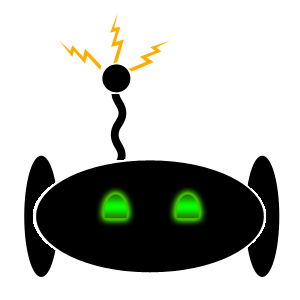
\includegraphics{logotyp.png}}
  	\end{picture}}
	
  \fancyhead[C]{\small{Mapmaster2001}}
  \fancyhead[R]{\small \today}
  \fancyfoot[L]{\small{TSEA56 \\ LIPS Kappa}}
  \fancyfoot[C]{\small{\thepage}}
  \fancyfoot[R]{\small{Projektgrupp 8 \\ mapmaster2001@cyd.liu.se}}

  %-----------------------------------------------------------------

%-------------------------------------------------------------------
%Första sidan

\MakePerPage{footnote} %the perpage package command footnotes need to restart on new sides

\begin{document}
	\pagestyle{fancy}
\pagenumbering{roman}
	\vspace*{\fill}
		\begingroup
			\begin{center}
				\huge{\textbf{Trådlös kommunikation}}
				\\
				\vspace{10pt}
				\normalsize
				Niklas Ericson och Jens Edhammer
				\\
				Kandidatprojekt Y - Grupp 8 - VT2014
				\\
				Version 1.0
				\end{center}
		\endgroup
	\vspace*{\fill}
	
	\begin{center} %Börjar centrering 
		Status
		\\
		\vspace{3pt} %Whitespace 3 pts
	    \begin{tabular}{| p{3cm} | p{3cm} | p{3cm} |} %tabell, 4 horizontella |, 3 cm emellan dem.
	    \hline %översta horizontella linjen.
	    Granskad & - & \today \\ \hline % & -tecken för att "gå till nästa ruta" 
		Godkänd & - & - \\ \hline % avslutas med \\ och \hline.

	    \end{tabular}
	\end{center}
	\vspace{2cm}
	\newpage
%-----------------------------------------------------------------
%Projektidentitet
	
	\vspace*{\fill}
		\begingroup
			\begin{center}
				\LARGE{\textbf{PROJEKTIDENTITET}}
				\\
				\footnotesize
				Grupp 8, 2014/VT, MapMaster2001
				\\
				Linköpings tekniska högskola, ISY
				\\
				\vspace{1cm}
	  \begin{tabular}{| p{3cm} | p{4.3cm} | p{2.4cm} | p{3.8cm} |}
	    \hline
		\textbf{Namn} & \textbf{Ansvar} & \textbf{Telefon} & \textbf{E-post} \\ \hline
	    Jens Edhammer & Dokumentanvsvarig (DOK) & 076-030 67 80 & jened502@student.liu.se \\ \hline
		Erik Ekelund & Designansvarig (DES) & 073-682 43 06 & eriek984@student.liu.se \\ \hline
		David Habrman &  & 976-017 71 15 & davha227@student.liu.se \\ \hline 
		Tobias Grundström & Testansvarig (TES) & 073-830 44 45 & tobgr602@student.liu.se \\ \hline 
		Hans-Filip Elo &   & 073-385 22 32 & hanel742@student.liu.se \\ \hline 
		Niklas Ericson & Projektledare (PL) & 073-052 27 05 & niker917@student.liu.se \\ \hline
	    \end{tabular}
		
		\vspace{1cm}
		\textbf{E-postlista för hela gruppen:} mapmaster2001@cyd.liu.se
		\\[0.5cm]
		
		\textbf{Kund}: Mattias Krysander, Linköpings Universitet, 581 83  LINKÖPING, \\
		013-28 21 98, matkr@isy.liu.se \\
		\textbf{Kontaktperson hos kund}: Mattias Krysander, 013-28 21 98,matkr@isy.liu.se 
		\\
		\textbf{Kursansvarig}: Tomas Svensson, 3B:528,013 28 21 59,tomass@isy.liu.se
		\\[0.5cm]
		\textbf{Handledare}: Peter Johansson, 013-28 1345 peter.a.johansson@liu.se

				\end{center}
		\endgroup
	\vspace*{\fill}
\newpage

%-----------------------------------------------------------------
%Innehållsföreteckning

\addto\captionsswedish{\renewcommand{\contentsname}{Innehållsförteckning}}

\tableofcontents
\thispagestyle{fancy}
\newpage

\pagenumbering{arabic}
%-----------------------------------------------------------------
%Översikt
\section{Inledning}
\section{Problemformulering}
\section{Principer för trådlös kommunikation}
\subsection{WLAN}
Ett wireless local area network (WLAN) kopplar ihop två eller flera noder med hjälp av någon form av trådlös distributionsmetod. Ett exempel på en sådan distributionsmetod är Orthogonal frequency-division multiplexing (OFDM) som utnyttjar olika bärvågfrekvenser får att koda om signalen. WLAN använder sig oftast av en accesspunkt så att noderna/användarna kan förflytta sig inom räckvidden för denna accesspunkt. Idag används mestadels WLAN som är baserade på standarden IEEE 802.11 som i vardagligt språk brukar kallas Wi-Fi. Standarden är skapat av Institute of Electrical and Electronics Engineers, (IEEE).

\subsubsection{Stationer}
Alla komponenter i ett WLAN utgörs av antingen stationer som kan vara noder eller accesspunkter. Alla stationerna har ett nätverkskort, wireless network interface controller (WNIC), som jobbar på samma lager som MAC-lagret (Se rubrik IEEE 802.11). Nätverkskortet använder antenn för att kommunicera med hjälp av radiovågor. En accesspunkt utgörs oftast av en router eller en switch medan en nod kan vara en PC eller mobiltelefon.

\subsubsection{IEEE 802.11}
IEEE 802.11 familjen består av en serie halv-duplex (kommunikationen kan ske i båda riktningarna men bara en riktning i taget) modulationstekniker som använder sig av samma MAC-protokoll. MAC-protokollet eller MAC-lagret är ett sublager i datalänklagret. Detta lager fungerar som en mellanhand mellan logical link control (LLC) och nätverkets fysiska lager och styr alltså hur nätverksnoderna får åtkomst till det fysiska skiktet (signal och binär överföring).
IEEE 802.11 kräver att nod \emph{x} konstant lyssnar för att vara redo om en nod \emph{y} möjligen skulle försöka skicka data. Detta drar givetvis mycket ström men kan reduceras med hjälp av en Network Allocatoin Vector (NAV), som enkelt sett fungerar som en räknare. När räknaren är nollskild är systemet i vila, när räknaren är noll så lyssnar systemet. Trådlösa stationer som har batteridrift kan därför spara ström genom att gå i vila och sen vakna till när räknaren är noll och då vara redo att ta emot data.\footnote{Holger Karl, Andreas Willig. Protocols and Architectures for Wireless Sensor Networks, Wiley, 2005}

\subsubsection{Säkerhet}
Användning av WLAN har ökat radikalt och blivit väldigt populärt på grund av dess flexibilitet och användarvänlighet, dock kommer dessa typer av nätverk alltid med lite säkerhetsrisker. IEEE 802.11 innehåller både kryptering och autentiserings metoder med hjälp av wired equivalent privacy (WEP).\footnote{Lopez-Aguilera, Elena. Study on the influence of transmission errors on RSNA authentication mechanisms in IEEE 802.11 WLAN. Computer Communications Volume: 41 Issue: 5 (2014-01-01) p. 76-93} Detta är en av de mest simpla metoder och har idag ersatts av  Wi-Fi Protected Access (WPA) som använder sig av en mer avancerad krypteringsmetod än WEP. 

\subsection{Bluetooth}

Bluetooth är en global standard för trådlöskommunikation på korta avstånd och utvecklades av Ericsson 1994. Bluetooth utnyttjades till en början primärt som en ersättning för serielkommunikationskablar mellan enheter.\footnote{\label{BTweb}Bluetooth SI. Fast Facts http://www.bluetooth.com/Pages/Fast-Facts.asp (Hämtad 2014-03-24)}
Bluetooth är fullt duplex och kan alltså skicka information i båda riktningar samtidigt. Dessutom kan Bluetooth sättas upp utan en tidigare existerande trådlös arkitektur och blir därför väldigt attraktiv för att para ihop enheter. Så som Bluetooth protokollet fungerar är det just parning mellan två enheter som är aktuellt. Bluetooth har fler aspekter som gör det särdeles bra för små mobila enheter.\footnote{\label{Gupta}Gupta, Naresh. Inside BLUETOOTH LOW ENERGY. Artech House, 2013}
\begin{itemize}
\item Låg strömförbrukning 
\item Låg kostnad
\item Liten formfaktor
\item Behöver ej fri sikt mellan enheterna
\end{itemize}

Bluetooth utnyttjar högfrekventa radio vågor mellan 2.4 GHz till 2.485 GHz för att sända information.$^{\ref{BTweb}}$

\subsubsection{Standarder för Bluetooth}
Hastighet för olika Bluetooth standarder:
\begin{itemize}
\item Bluetooth 1.2 - 1 Mbit/s 
\item Bluetooth 2.0 - 3 Mbit/s
\item Bluetooth 3.0 - 24 Mbit/s
\item Bluetooth 4.0 - 24 Mbit/s
\end{itemize}

Intressant att notera här är att Bluetooth 3.0 har en teoretisk överföringshastighet på 24 Mbit/s, men att denna överföring inte sker via Bluetooth, utan via den snabbare teknologin IEEE 802.11. 
Bluetooth 4.0 ökar inte hastigheten från 3.0 utan fokuserar istället på att spara in på strömförbrukning.$^{\ref{Gupta}}$


\subsubsection{Koppling av enheter}
En parkoppling mellan två Bluetooth-enheter, A och B, fungerar enligt principen att ena enheten, låt oss säga enhet B, måsta vara upptäckbar och måste alltså sända ut en form av identifikation, ofta i form av ett namn. Enhet A söker av vilka enheter den kan detektera och ger ofta en komplett lista till användaren över enheter som den detekterade. Nästa steg är att enhet A begär en koppling till enhet B. När kopplingen lyckas blir enhet A master och enhet B slave. Tvåvägskommunikation är nu möjlig mellan enheterna.\footnote{\label{Gupta2}Gupta, Naresh. Inside BLUETOOTH LOW ENERGY. Artech House, 2013}

\subsubsection{Säkerhet}
Bluetooth är en förhållandevis säker kommunikationsform, men är självklart inte helt säker. En begränsning i säkerheten är att Bluetooth-enheterna ofta saknar inmatningsmöjligheter och display. Detta leder till att lösenord inte kan fyllas i eller ens genereras på enheterna. I fallet av att båda enheter har display och inmatningsmöjligheter kan en 16 siffror lång PIN-kod genereras som sedan måste fyllas i på den enhet som begär kopplingen. Detta skyddar mot de flesta former av avlyssning.
För enheter som saknar antingen display eller inmatningsmöjligheter finns andra möjliga lösningar. NFC alltså Near-Field Communication, kan användas för parning och då måste enheterna i princip röra varandra i parningsfasen men kan därefter utnyttja fulla räckvidden på Bluetooth. Detta kallas Out-of-Band Pairing.$^{\ref{Gupta2}}$

En annan typ av säkerhet som används är ''Just Work'', som utnyttjas när enheterna saknar både inmatningsmöjligheter och display. Ett exempel på detta är Bluetooth headsets till mobiltelefoner. Denna säkerhetsmetod kräver inte att användare utför någonting förutom själva kopplingen. Denna metod skyddar mot passiv avlyssning, men ej mot aktiv avlyssning. 
Aktiv avlyssning är när en enhet lägger sig mellan de två enheterna och vidarebefodrar kommunikationen emellan dem och kan vara väldigt svår att upptäcka.
Passiv avlyssning så försöker man endast lyssna av kommunikationen mellan två enheter.$^{\ref{Gupta2}}$
 
\subsection{Infrared (IR)}
IR kommunikation är en form av trådlös kommunikation där informationen skickas i form av IR-ljus och kräver därför direkt siktlinje mellan sändare och mottagare. En vanlig implementering av denna form av kommunikation är fjärrkontroller till TV-apparater.
Infrared Data Association Standards (IrDA) är en assosciation bestående av ungefär 100 medlemsföretag. IrDA protokollen är ett såkallat Point-to-Point protokoll och skickar alltså kommunikation mellan två enheter. IrDA har överföringshastighet på 2.4 kb/s upp till 4 Mb/s på upp till 1 meters avstånd. Vid länkning av två enheter kommer dessa alltid att kommunicera med 9.6 kb/s för att sedan komma överens om vilken hastighet som ska köras under dataöverföring.\footnote{\label{Carruthers}Carruthers, Jeffrey B. Wireless Infrared Communications,Department of Electrical and Computer Engineering
Boston University, 2002, http://iss.bu.edu/jbc/Publications/jbc-bc1.pdf (Hämtad 2014-03-24)}  

\subsubsection{Långdistans IR kommunikation}
Flera hinder finns för konstruktion för långdistans kommunikation via IR. Dessa enheter behöver fri sikt och lider av signalstyrke förlust genom atmosfären.$^{\ref{Carruthers}}$ 

\subsubsection{Säkerhet}
Säkerhet i IR-kommunikationsfallet vid kortdistans fallet faller mer eller mindre under det faktum att avstånden för överföring är såpass små att hackningförsök blir inaktuella.$^{\ref{Carruthers}}$

\subsection{ZigBee}
ZigBee är en standard för trådlös styrning och övervakning som används i hem och industrier men även andra övervaknings och styrningsapplikationer där låg strömförbrukning och hög tillgänglighet är i fokus. Zigbee-standarden erbjuder näverks-, säkerhets- och applikationssupport ovanpå IEEE 802.15.4 standarden. Platformen har stöd för stjärnnät och trädstruktur men mesh-arkitektur är den absolut populäraste. 

\subsubsection{IEEE 802.15.4}


\subsubsection{Mesh-arkitektur}
Mesh-arkitekturen är en nätstruktur där alla noder i nätet har kontakt med minst 2 noder samtidigt. Detta ger i sin tur ger i sin tur hög redundans vilket leder till högre säkerhet på kommunikationen. Strukturen är således tillförlitlig och erbjuder bra skydd mot varianser i signalstyrka som kan skapas av interferens eller multipla signaler.\footnote{Wheeler, Andy. Krama saften ur Zigbee. Elektronik Tidningen (2005).(Hämtad 2014-03-24)}


\subsection{Radiostyrning}
\section{Resultat}
\subsection{Diskussion}

Disposition: 
\\
1. Inledning 
\\
2. Problemformulering (frågeställningar som rapporten ska behandla) 
\\
3. Kunskapsbas (litteratur, datablad, dokumentation, etc.) 
\\
4. Fördjupningstext (modeller, beräkningar, analyser och eventuella experiment) 
\\
5. Resultat och slutsatser 





% ----------------------------- Appendix -----------------------------------------

\newpage
\appendix
Författare:Gupta, Naresh C. (Naresh Chand), Titel Inside Bluetooth Low Energy Utgivare:Artech House,Utgivningsdatum:cop. 2013Sidor:xxvi, 395 pages :ISBN:9781608075799
\pagestyle{empty}
\newgeometry{left=2cm,right=2cm,bottom=2cm,top=2cm}
\section{Referenser}
%http://etn.se/index.php?option=com_content&task=view&id=18463&Itemid=66


\end{document}